\chapter{Title to be decided}
\label{capitolo4}
\thispagestyle{empty}

\section{Basics}
\noindent The purpose of this work is to create a computer program that is able to deeply understand solar data in order to accurately estimate the sunspot index. To do that, we have to train our computer to mimic the reasoning of one or more human experts. In simpler words, our purpose is to develop a model that is capable of \textit{learning}. One can ask himsef if the fact that a program is able to learn implies some kind of \textit{``intelligence''} underneath. The answer depends on how the concept of intelligence is defined. Arguably, regardless of filosophical questions, this thesis can be said to belong to the field of Artificial Intelligence. The latter is essentially the field that builds artificial algorithms that process information in order to make future decisions. A large subset of this family of algorithms is called Machine Learning. Machine Learning is the discipline that studies how to provide computers with the ability to learn and improve their preformance over time automatically. It is usually divided into three main subfields: supervised learning, unsupervised learning and reinforcement learning. However, since reinforcement learning is out of the scope of this thesis, we will focus on the former two. \\
The goal of supervised learning is to find the function that best approximates the desired outputs given some input data. What is interesting about this function approximation task is that it can be done without explicitly instructing the program (also called model) on how to do it, but instead letting it learn useful patterns from experience. This process is referred to as supervised because the model is not free to choose its own experience, but rather uses the data itself, in the form of inputs and outputs. In the learning of this mapping, we also expect the algorithm to generalize from the training to unseen situations in a reasonable way, not simply memorizing each and every data point it is fed (overfitting). Specifically, translating this idea to the real task of sunspot counting, it is desirable to build an agent that, after being taught by the experts on how to label images of the Sun, will be able to perform it automatically.\\
The second step of our algorithm tackles the problem of partitioning sunspot into groups. That's where unsupervised learning comes into play. The set-up of the problem is similar to the previous case, you have some data and want to teach a model to find interesting patterns in it, in order to perfom some task. The crucial difference is that the data is not labeled. In other words, compared to the supervised setting, this means that the output data is missing. Therefore, instead of learning a mapping, the goal for unsupervised learning is to model the underlying structure in the data to extract more insights about it. Examples of unsupervised learning techinques that will be treated in this thesis are clustering and representation learning.\\
Orthogonally to these three macro-categories, Machine Learning encompasses a plethora of models, each one with its strenghts and weaknesses. This work focuses on the type of model that is most popular at the time of writing: the Artificial Neural Network, a computing paradigm that was inspired by biological neural networks that constitute human brains. They consist of artificial neurons organized in layers that communicate with each other by sending signals. Each neuron is nothing more than a mathematical function with $m$ inputs that computes the following:
\begin{equation}
y = f \left(\sum_{j=0}^{m} w_{j}x_{j}\right)
\end{equation}
Where $f$ is an activation function and $w$ is the vector containing the weight for every input $x$. Also, $x_0$ is a special input, called \textit{bias}, whose value is fixed to 1. This allows the activation function to be shifted to the left or to the right, to better fit the data. Changes to the weights alter the steepness of the activation function, while the bias offsets it. The blocks composing the artificial neuron can be schematized as below: \\
\begin{center}
  \begin{tikzpicture}[
  init/.style={
    draw,
    circle,
    inner sep=2pt,
    font=\Huge,
    join = by -latex
  },
  squa/.style={
    draw,
    inner sep=2pt,
    font=\Large,
    join = by -latex
  },
  start chain=2,node distance=13mm
  ]
  \node[on chain=2]
    (x2) {$x_2$};
  \node[on chain=2,join=by o-latex]
    {$w_2$};
  \node[on chain=2,init] (sigma)
    {$\displaystyle\Sigma$};
  \node[on chain=2,squa,label=above:{\parbox{2cm}{\centering Activation \\ function}}]
    {$f$};
  \node[on chain=2,label=above:Output,join=by -latex]
    {$y$};
  \begin{scope}[start chain=1]
  \node[on chain=1] at (0,1.5cm)
    (x1) {$x_1$};
  \node[on chain=1,join=by o-latex]
    (w1) {$w_1$};
  \end{scope}
  \begin{scope}[start chain=3]
  \node[on chain=3] at (0,-1.5cm)
    (x3) {$x_3$};
  \node[on chain=3,label=below:Weights,join=by o-latex]
    (w3) {$w_3$};
  \end{scope}
  \node[label=above:\parbox{2cm}{\centering Bias \\ $x_0=1, w_0$}] at (sigma|-w1) (b) {};

  \draw[-latex] (w1) -- (sigma);
  \draw[-latex] (w3) -- (sigma);
  \draw[o-latex] (b) -- (sigma);

  \draw[decorate,decoration={brace,mirror}] (x1.north west) -- node[left=10pt] {Inputs} (x3.south west);
  \end{tikzpicture}
\end{center}
\begin{figure}[b!]
  \centering
  \caption{Multi-layer fully connected network architecture}
  \label{fig:mlfc}
  \def\layersep{2.5cm}
  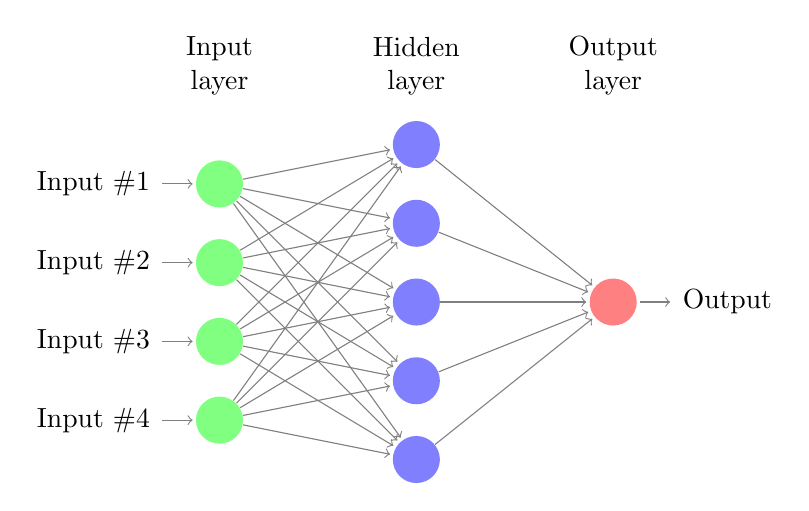
\begin{tikzpicture}[shorten >=1pt,->,draw=black!50, node distance=\layersep]
      \tikzstyle{every pin edge}=[<-,shorten <=1pt]
      \tikzstyle{neuron}=[circle,fill=black!25,minimum size=17pt,inner sep=0pt]
      \tikzstyle{input neuron}=[neuron, fill=green!50];
      \tikzstyle{output neuron}=[neuron, fill=red!50];
      \tikzstyle{hidden neuron}=[neuron, fill=blue!50];
      \tikzstyle{annot} = [text width=4em, text centered]

      % Draw the input layer nodes
      \foreach \name / \y in {1,...,4}
      % This is the same as writing \foreach \name / \y in {1/1,2/2,3/3,4/4}
          \node[input neuron, pin=left:Input \#\y] (I-\name) at (0,-\y) {};

      % Draw the hidden layer nodes
      \foreach \name / \y in {1,...,5}
          \path[yshift=0.5cm]
              node[hidden neuron] (H-\name) at (\layersep,-\y cm) {};

      % Draw the output layer node
      \node[output neuron,pin={[pin edge={->}]right:Output}, right of=H-3] (O) {};

      % Connect every node in the input layer with every node in the
      % hidden layer.
      \foreach \source in {1,...,4}
          \foreach \dest in {1,...,5}
              \path (I-\source) edge (H-\dest);

      % Connect every node in the hidden layer with the output layer
      \foreach \source in {1,...,5}
          \path (H-\source) edge (O);

      % Annotate the layers
      \node[annot,above of=H-1, node distance=1cm] (hl) {Hidden layer};
      \node[annot,left of=hl] {Input layer};
      \node[annot,right of=hl] {Output layer};
  \end{tikzpicture}
\end{figure}
\noindent As the reader can verify, the final decision about the magnitude of the signal is taken by the activation function. It is resposible to determine whether or not the input features are important enough to further contribute to the computation. The activation is a non-linear function, generally continuous and differentiable (except for very primitive formulations, like the perceptron \cite{rosenblatt1961principles}). These two properties are fundamental to build a multi-layered architecture. In fact, imagine to stack more than one layer of neurons as in Figure~\ref{fig:mlfc} where the output of the neurons are attached as inputs to the subsequent layer, then ideally, the larger the number of layers, the more ``learning power'' the network attains. Now, if the activation function was simply linear, regardless of how many layers are stacked, there would exist a single neuron that could approximate the same function, because the composition of linear functions is always just linear. Non-linearity solves this problem and enables deep architectures. But how do these artificial networks learn? Through trial and error, in a way that is arguably similar to the process of human learning. First, the inputs get propagated forward through the neurons until the output layer is reached and then the error is calculated with respect to the desired output value using a loss function. Intuitively, the loss represents the cost of the error, or a measure of the penalty the network will experience. Therefore, learning can be seen as an optimization problem that seeks to minimize the loss as objective function. The last building block needed for the network to improve its performance over time is the weight update through backpropagation (short for ``backward propagation of errors''). In fact, the weights of the neurons have a relationship with the error the network produces, thus, if the parameters make an adjustment in the right direction, the error decreases. The direction of the update is usually calculated by means of an optimization algorithm called gradient descent, that is based on the observation that a function decreases fastest if one goes in the direction of the negative gradient. Hence, given a learning rate $\gamma$ small enough, the loss $\mathcal{L}$, a weight vector $\theta$ and the following update:
\begin{equation}
  \theta_j \leftarrow \theta_j - \gamma\frac{\partial \mathcal{L}}{\partial \theta_j}
\end{equation}
then the loss is guaranteed to decrease. However, in the real case the learning rate is fixed so it is not mathematically certain that the performance will improve at each and every step, although it still works well in practice.\\
Neural networks are a very flexible tool that can be used for virtually every problem, yielding good performance. Neurons can be connected to each other in many ways, forming several architectures, in order to adapt them to different data types (images, sentences, etc.). Also, they can be used with good results in all the subfields of machine learning. The following two sections will explain how to build neural networks that are capable of processing images in both supervised and unsupervised settings.

\section{Semantic Segmentation}
Image segmentation is the partitioning of an image into several groups of pixels, also called segments, based on some criteria. The segments of an image are usually stored in a mask where each group is assigned a unique grayscale value or color to identify it. Image processing solutions to this problem, employing a wide range of criteria, have been deeply explored. Sometimes, it is posed as a graph partitioning problem \cite{shi2000normalized}, other times as a clustering task \cite{coleman1979image}. However, in general, these criteria do not make any attemps at understanding what the segments represent.\\
\begin{figure}[t]
    \centering
    \includegraphics[width=\textwidth]{./pictures/segmentation-masks}
    \caption{Examples of Semantic segmentation.}
    \label{fig:segmentation-masks}
\end{figure}\\
With the rise of Computer Vision the situtation changed completely. Instead of just applying some transformations to the image, Computer Vision aims to extract knowledge from the scene. Pixels are no longer seen as mere elements in a matrix, but rather as a means of conveying meaning. Performing image segmentation based on the understanding of the content is called semantic segmentation. Back in the 1990s, segmentation was carried out using probabilistic frameworks, like conditional random fields (CRFs) among the others. Their advantage is that they can model the relationship between pixels in order to be more accurate in the prediction of the label. Nowadays, CRFs are not really used anymore, except as post-processing step of neural network models. In fact, around 2006, a group of researchers brought together by the Canadian Institute for Advanced Research (CIFAR) showed that it is possible to train very deep artificial neural networks effectively \cite{hinton2006fast} and that they outperform any other algorithm on computer vision tasks \cite{hinton2006reducing}. It was the dawn of the Deep Learning era. The following years saw a rapid increase in the quantity of scientific articles using deep neural networks, tackling all sorts of problems that, until then, seemed unsolvable.
In the context of semantic segmentation this revolution led to the invention of fully convolutional networks (FCNs - Long et al.\cite{long2015fully}), a particular flavour of neural architecture that is able to produce pixel-level classification. Actually, the idea of using convolution-like operations to feed pixels into neurons first emerged in 1980 \cite{fukushima1980neocognitron} and ways of training them through backpropagation ware proposed around ten years later \cite{waibel1995phoneme}\cite{lecun1989backpropagation}.
Convolutional Neural Networks (CNNs) take advantage of the fact that the input consists of images and they constrain the architecture in a more sensible way. In particular, unlike a regular neural network, the layers (or filters) of a CNN have neurons arranged in 3 dimensions: width, height and depth (Figure~\ref{fig:conv-layer}). The neurons in a layer will only be connected to a small region of the layer that precedes them, instead of collecting the activations of all neurons in a fully connected manner \cite{cnn-stanford}. Using this trick has 2 advantages, first, it decreases the number of parameters to be learned by a large margin, second, it forces the model to learn hierarchically, concentrating on smaller regions of the image to capture local information, but then merging them together to deduce more high-level concepts. In practice, a CNN is able to encode the content of an image, automatically extracting features that are very effective at discriminating between classes, while at the same time preserving spacial information. This characteristic is fundamental because semantic segmentation faces an inherent tension between semantics and location: global information resolves ``what'' while local information resolves ``where''\cite{long2015fully}.
\begin{figure}[t]
    \centering
    \includegraphics[width=\textwidth]{./pictures/conv-layer}
    \caption{A visualization of a Convolutional Neural Network. In red the input image, in blue the convolutional layers, in green the output layer \cite{cnn-stanford}.}
    \label{fig:conv-layer}
\end{figure}
A FCN leverages the strenghts of this convolution-like operation to create an encoder-decoder architecture that is able to predict the location and the class of each object in the input. The encoder is a stack of convolutional, max pooling and batch normalization layers, where max pooling is a down-sampling operation that keeps the largest value, and batch normalization \cite{ioffe2015batch} handles the adjusting and scaling of the activations. The decoder is built similarly, but it up-samples the coarse feature maps into a full-resolution segmentation map using the transpose operation. The transpose convolutional filter does the opposite of a normal one, instead of performing a weighted sum of the inputs, it takes a single value, multiplies it by the weights of the filter and spreads the output values in the neighboring region of the next layer. Long et al. also added ``skip connections'' that take activations from the encoder and sum them up to the up-sampled features of the decoder. The information extracted from earlier layers in the network (prior to a down-sampling operation) should provide the necessary detail in order to reconstruct accurate shapes for segmentation boundaries.\\
\begin{figure}[t]
    \centering
    \includegraphics[width=\textwidth]{./pictures/u-net}
    \caption{U-Net architecture \cite{ronneberger2015u}.}
    \label{fig:unet}
\end{figure}\\
So, at training time, the network takes an image as input and propagates the values forward through the encoder and the decoder, until the output layer is reached. Subsequently, the error is calculated and the whole network is updated end-to-end using backpropagation. The loss function that leads the training should be carefully chosen, depending on the architecture and the specific problem that is being dealt with. However, in general, the good old cross entropy loss over each pixel can be used for segmentation:
\begin{equation}
\mathcal{L}(p, y) = -y\log(p)-(1-y)log(1-p)
\end{equation}
where $p$ is the predicted probability that a pixel belongs or not to the class and $y$ is the ground truth. This measure is a solid choice with regard to image segmentation, because it returns very stable gradients to the network and helps it converge smoothly. However, in some cases, cross entropy doesn't correlate well with human perception, especially when the distribution of the classes in the dataset is highly imbalaced. For this reason, other loss functions were introduced in the deep learning field. One of them is the Dice loss \cite{sudre2017generalised}, based on the Dice coefficient ($DC$) \cite{sorensen1948method}\cite{dice1945measures}, in formulas:
\begin{equation}
DC(X,Y) = \frac{2|X\cap Y|}{|X\cup Y|}
\end{equation}
where $X$ and $Y$ are respectively the set of pixels belonging to the predicted mask and the ground truth mask. Doing so, this coefficient quantifies the similarity (or overlap) between the real distribution of the classes and the one that was estimated by the network. \\
Among all the architectural proposals that followed the first FCN article \cite{long2015fully}, the one that most impacted the field was the U-Net \cite{ronneberger2015u}. Ronneberger et al. improve upon the vanilla version of the FCN primarily through improving the capacity of the decoder module of the network. More concretely, the strength of the U-Net consists in its symmetry, in other words the contracting path and the expanding path have roughly the same depth. In addition, the skip connections are revisited, in fact, in this architecture the features of the encoder are not summed to the ones of the decoder but rather concatenated. Thanks to these adjustments the U-Net produces much better results, being capable of distinguishing the details of objects from the background noise.\\
Over time, a wide range of more advanced atomic blocks got discovered and substituted to the original CNN blocks. This led to the pubblication of new versions of the U-Net. For example, in 2016, residual blocks \cite{he2016deep} were added to the architecture \cite{drozdzal2016importance} allowing faster convergence and deeper models to be trained. However, the simple but powerful ideas that laid the foundations for the U-Net still make it a very solid choice.

\section{Clustering}
Clustering is the process of identifying natural groupings or clusters within multidimensional data, based on some similarity measures \cite{omran2007overview}. Clusters differ from classes because they are not known a priori but they are rather extracted from the data. Clustering can be achieved by various algorithms that differ significantly in the way they model the data. Despite this, all of its various realizations belong to the unsupervised learning family. \\
The purpose of this section is not to compile a review of each and every clustering algorithm. For that, the reader should refer to the extensive literature on the topic that can be found in bibliography \cite{omran2007overview}\cite{jain1999data}. This section is more of a brief overview on the methods that will be used in our main algorithm and the more subtle tweaks that make clustering work well.\\
Broadly speaking, clustering can be divided into two subgroups: those that require a priori knowledge of the number of clusters and those that are able to infer it. This distincion is particularly important in the context of sunspot detection because humans are very good at deducing the number of sunspot groups intuitively. An example of an algorithm that needs to know the number of clusters before running is k-means. Became very popular because of its simplicity and efficiency, K-means belongs to the type of algorithms that model clusters as centroids. In fact, it initializes $k$ randomly selected centroids which are used as the beginning points for every cluster, and then performs iterative calculations to finding the least-squares assignment to centroids. The algorithm terminates when the centroids have stabilized or alternatively when the maximim number of iteration has been reached. K-means, as most clustering algorithms, is not guaranteed to return the globally best solution. To mitigate this issue, the procedure can be restarted randomly for a fixed number of times. Although k-means is not able to determine the number of clusters automatically some methods have been developed in order to fix this, like the silhouette method \cite{rousseeuw1987silhouettes} or the elbow method.
\begin{figure}[b!]
    \centering
    \includegraphics[width=\textwidth]{./pictures/dbscan}
    \caption{A visualization of DBSCAN running. Core points are highlighted in red, border points in yellow, outliers (noise) in blue}
    \label{fig:unet}
\end{figure}\\
\noindent In the panorama of clustering algorithms that do not require a prior estimate of the number of clusters, DBSCAN \cite{ester1996density} is one of the most famous. DBSCAN is based on a very different premise with respect to k-means. In fact it defines the clusters as dense connected regions in the data space. It takes 2 parameters as input:
\begin{itemize}
  \item \textbf{eps} ($\varepsilon$): the minimum distance between two points for them to be considered neighbors;
  \item \textbf{minPts}: the minimum number of points to form a dense region (core).
\end{itemize}
So, what happens at runtime is that a point is drawn from the dataset, DBSCAN forms an n-dimensional shape with radius $\varepsilon$ around that data point, and then counts how many data points (neighbors) fall within that shape. If the number of neighbors is at least \textit{minPts} then the selected point belongs to the core, otherwise it can be labeled as a border point or an outlier. Neighbors get expanded as well and the process continues until the density-connected cluster is completely found. Then, a new unvisited point is drawn and the same routine is repeated. The resulting clustering has the property that all the clusters have at least density $\varepsilon$. Therefore, DBSCAN works well under the assumption that the density of the clusters is homogeneous. Also, one of the advantages of using density is that it can be calculated using virtually any metric, while, by contrast, algorithms like k-means assume the points lay in an euclidean space. In any case in this thesis we will feed such algorithms with data representations learned to optimize their distribution in a euclidean space.

\section{Representation Learning}
Every day, when we read, hear a noise, see an object or, in other words, experience the world through senses our brains are flooded by information. One of the astonishing aspects of our intelligence is that we do not drown in this massive flow of data, but rather we are able to navigate through it. Much of the ability to draw the best from our perceptions is due to the way we represent information. In the human brain, sensory information is represented by neural activity. Recent studies proved that using the distribution of activation in the neural population generated by the sight of some object it is possible to reconstruct an image of the object itself \cite{shen2019deep}. This result suggests that the brain is constantly extracting salient features from perceptions.\\
Unsurprisingly, representation learning (also known as feature learning) is a fundamental step in almost any machine learning pipeline. Learning a representation means to find a model that maps a generic data point in a high-dimensional space to a set of latent variables in a low-dimensional space. Latent variables, as opposed to observable variables, are variables that are not directly observed but rather inferred. This feature transformation technique can be very useful because depending on how data is represented, different information can be uncovered. Nontheless, it is rarely used as a stand-alone procedure. To make the most out of it, representation learning should be coupled with other supervised or unsupervised techinques. In fact a good representation is one that makes a subsequent learning task easier \cite[Chapter~15]{goodfellow2016deep}.\\ % The choice of representation will usually depend on the choice of the subsequent learning task.
Many different approaches to representation learning are possible and some of them will be described here. The most straightforward way of discovering good descriptors for the data is through unsupervised learning. A statistical approach to representation learning is offered by the Principal Component Analysis (PCA) algorithm \cite{jolliffe2011principal}. PCA is a dimensionality reduction algorithm that uses an orthogonal transformation to convert a set of observations of possibly correlated variables into a set of linearly uncorrelated variables called principal components. The first principal component accounts for as much of the variability in the data as possible, and each succeeding component accounts for as much of the remaining variability as possible. Representations can be extracted from the principal components and used as inputs to other models. PCA is very popular and effective in some situations, but suffers many limitations due to the assumptions that is makes. One of the most criticized aspects is that it can only find linear correlations, but the relationships among data aren't always so simple. This assumption can be relaxed using models that are capable on non-linearity. Autoencoders are an example of this. They are particular types of neural networks that try to reconstruct their input. As in the case of image segmentation models, the architecture is composed by an encoder and a decoder, however, the interesting part here is not the output, but the bottleneck. The encoder is forced to produce a representation of the input that carries as much information as possible, in order for the decoder to be able to reconstruct the input. The features that are sampled at the bottleneck of the network can have several different properties, depending on the activation function and the loss that are used. Autoencoders can be used in combination with convolutional blocks as well, in order to extract features from images.\\
Clustering can also be considered an unsupervised feature learning algorithm. In fact, imagine to run, for instance, k-means on a dataset. The procedure will return $k$ centroids, where $k$ is the desired number of clusters. Features can be produced in several ways from the centroids. The simplest is to create a $k$-dimensional one-hot vector for each data point, where the $j$-th element of that vector is $1$ if the point belongs to the $j$-th cluster. It is also possible to use the distances to the clusters as features.\\
The situation changes when we have more information about the problem we want to solve. In fact we can train supervised learning models that look for the exact characteristics of the data that are most important to separate some predefined class. Imagine to have a dataset with 10 classes and to know the class associated to each record. Ideally, it is possible to train a model that is capable of taking two records as input and calculating their similarity. The model will be trained using the information about the classes as a supervision signal, for example the similarity can be defined to be $1$ when both inputs belong to the same class and $0$ otherwise. Once the model has converged, it can be used to predict the structure in unseeen data. In fact, there is plenty of clustering algorithms that are capable of taking a similarity matrix and find the clusters that optimize some measure. Hopefully then, each cluster will be trivially associated to the right class. This looks like a very far fetched approach in this case, because there are only 10 classes. With a low number of classes it is much easier to build a classifier that discerns them. But suppose to be working on Facebook's dataset of faces, where millions of people are catalogued. In this latter case, the classifier approach becomes unfeasible because it would have to decide among millions of classes, making complexity explode. On the other hand, for the similarity model this is not a problem, it just has more data to be trained on. In fact, pairwise similarity is still well defined and the large matrix that holds it doesn't have to be necessarily precomputed for the clustering phase. In practice, this model creates a different data representation by exploiting the relationships between the records. The new representation is indeed the similarity matrix.
\begin{figure}[b!]
    \centering
    \includegraphics[height=0.6\textheight]{./pictures/siamese}
    \caption{Siamese network architecture.}
    \label{fig:siamese}
\end{figure}\\
Several new studies elaborated on the concept that relative knowledge is, sometimes, a very powerful source to be drawn from. In the field of computer vision the solution to the problem of learning similarities in the data is called siamese network \cite{koch2015siamese}. The siamese network is a class of neural architectures that contain two or more identical subnetworks. Identical here means every aspect is shared, they have the same configuration, parameters and weights. In the case of two subnetworks, at training time each one takes one of the two input images and encodes it in a vector representation, also called embedding. The two outputs are then fed to a contrastive loss function \cite{hadsell2006dimensionality} defined as follows:
\begin{equation}
  \mathcal{CL}(D_{W_{12}}, y, m) = (y)\frac{1}{2}D_{W_{12}}^2 + (1-y)\frac{1}{2}max(0,m-D_{W_{12}})^2
\end{equation}
where $D_{W_{12}}$ is the distance between embedding $W_1$ and $W_2$, $y$ is the ground truth of the similarity and $m$ is the margin hyperparameter. The loss is called contrastive because it forces the model to learn how to embed images in such a way that neighbors are pulled together while, by contrast, non-neighbors are pushed apart. As the weights evolve during the training the updates are mirrored across both subnetworks. At testing time, all the images are embedded so that data becomes just a set of feature vectors. Any type of supervised or unsupervised learning algorithm can subsequently leverage the general representations generated by siamese networks. However, we will mainly focus on clustering methods that are able to group together all the realization of the same class in the test set. Representations can be learned in a way that optimizes clustering performance. It is sufficient to align the type of distance that is used by the contrastive loss and the clustering. So if, for instance, the distance $D_W$ in the loss is euclidean, then the clustering should be tuned accordingly to consider that the points lay in an euclidean space. Moreover, if the number of classes in the test set is not known a priori knowing the expected distance between the clusters could be very useful. Here the parameter $m$ comes into play. In fact, $m$ represents the margin after which the network won't push two dissimilar points further apart. It is therefore reasonable to assume that the expected distance between clusters will be roughly $m$.\\
Nowadays, the state of the art results for siamese networks are achieved using a slightly different version of the contrastive loss: the triplet loss. While the contrastive loss aims at relativey minimizing and maximizing the distance between similar (positive) and dissimilar (negative) examples separately, the triplet formulation does both things at the same time. Formally:
\begin{equation}
  \mathcal{TL}(D_{W_{ap}},D_{W_{an}}, m) = max(0,m+D_{W_{ap}}-D_{W_{an}})
\end{equation}
Where $D_{W_{ap}}$ is the distance between the anchor and and the positive example, $D_{W_{an}}$ between the anchor and the negative and $m$ is, again, the margin. The advantage with respect to the normal contrastive formulation is that, updating on both positive and negative cases concurrently you can manage to be less greedy, or alternatively to take into account more context. That said, sampling heuristic in such pairwise distance learning setting may be as crucial as choosing the right loss, as some studies state \cite{wu2017sampling}.

% \section{Complementary Methods}
% Deep neural networks are still very obscure and it is not straightforward to fully harness their power. Therefore, researchers came up with very ingenious stratagems to make them converge. In this section, some of the strategies that are currently being used to improve neural performance will be presented.
% \subsection{Optimizers}
% As already mentioned in this chapter, neural networks learn by an optimization algorithm called gradient descent. Yet, just using the vanilla version of it won't make the networks learn properly. Convergence can be slow for functions whose curvature varies chaotically depending on which direction the gradient points. Also, it causes the model to be very sensitive to the choice of the value of the learning rate, making the learning process unstable. Stochasting gradient descent (SGD) is an optimizer that builds upon gradient descent replacing the real gradient with a stochastic approximation. Instead of calculating the gradients for all of the training examples, it is sometimes more efficient to only use a random subset of these examples. By doing so, it increases the noise on the gradient but at the same time it acts like a regularizer to the gradient estimation, removing the bias of the training set. Regardless of stochasticity, a very simple way to accelerate optimizers is to introduce momentum. Rather than using only the gradient of the current step to guide the search, momentum also accumulates the gradient of the past steps to determine the direction to go. Adam \cite{kingma2014adam} combines adaptive momentum, SGD and other techniques to create the currently most used optimizer.
% \subsection{Multitask Learning}
% Convergence on very challenging tasks can be difficult and require a lot of computational resources. To accelerate the learni up Transfer Learning only aims at achieving high performance in the target task by transferring knowledge from the source task
% Rich Caruana defines multi-task learning as ``Multitask Learning is an approach to inductive transfer that improves generalization by using the domain information contained in the training signals of related tasks as an inductive bias. It does this by learning tasks in parallel while using a shared representation; what is learned for each task can help other tasks be learned better''\cite{caruana1997multitask}
% In the context of deep neural networks, multitask learning is achieved by architectures that have a bunch of shared layers and then task specific layers.
% Humans reuse knowledge from among different tasks to solve another task.
%
% shared features double check
% \subsection{CoordConv}
